\documentclass[aspectratio=169]{beamer}
\usepackage{amsmath, amsfonts, epsfig, xspace}
\usepackage{algorithm,algorithmic}
\usepackage{pstricks,pst-node}
\usepackage{multimedia}
\usepackage[normal,tight,center]{subfigure}
\setlength{\subfigcapskip}{-.5em}
\usepackage{beamerthemesplit}
\usetheme{keynote}
\usepackage{color}
%this is for the \hl{} highlight command 
\usepackage{soul}
%This makes it able to use different colours using \hlc[colourname]{}
\newcommand{\hlc}[2][yellow]{ {\sethlcolor{#1} \hl{#2}} }
%This is for framing text
\usepackage{framed}
\definecolor{shadecolor}{RGB}{255,127,0}

%----------Customize Title--
\defbeamertemplate*{title page}{customized}[1][]
{
  \begin{shaded}
  \usebeamerfont{title}\inserttitle\par
  \end{shaded}
  %\usebeamerfont{subtitle}\usebeamercolor[fg]{subtitle}\insertsubtitle\par
  %\bigskip
  %\usebeamerfont{author}\insertauthor\par
  %\usebeamerfont{institute}\insertinstitute\par
  %\usebeamerfont{date}\insertdate\par
  \usebeamercolor[fg]{titlegraphic}\inserttitlegraphic
}

%----------Beamer Modes---
%These modes are loaded with \mode<mode name>. They may
%also appear in the <overlay specification> option in the
%\begin{frame} command or as an option to the
%\documentclass.
%\modebeamer %(default)
%\modepresentation
%\modehandout
%\modetrans %(transparencies)
%\modearticle
%\modeall
%----------Print Handouts---
%To produce handouts, change the \documentclass command to
%\documentclass[handout]{beamer} and add
%\usepackage{pgfpages} This disables hyperlinks.
%\pgfpagesuselayout{4 on 1} Puts 4 slides on each page.
%\setbeamertemplate{navigation symbols}{} Turns on
%navigation bars at the bottom of each slide.
%----------Hacks-----------------
%http://www.shawnlankton.com/2008/02/beamer-and-latex-with-keynote-theme/
%\titlegraphic{
\includegraphics[height=1cm]{iwmi}}
%\pgfdeclareimage[height=0.5cm]{iwmi}{iwmi}
%\logo{\pgfuseimage{iwmi}}
\setbeamercolor{titlelike}{parent=structure,fg=white}
%-----------------------------------

\title[JRC\hspace{2em}\insertframenumber/\inserttotalframenumber]{MonSTERS Wars \\Episode MMXVII-III-XXIII\\\textit{The Separation of the Crowns}}
\author[Yann Chemin]{Yann Chemin}
\institute{JRC}
\date{} %leave out for today's date to be insterted

\begin{document}

{\usebackgroundtemplate{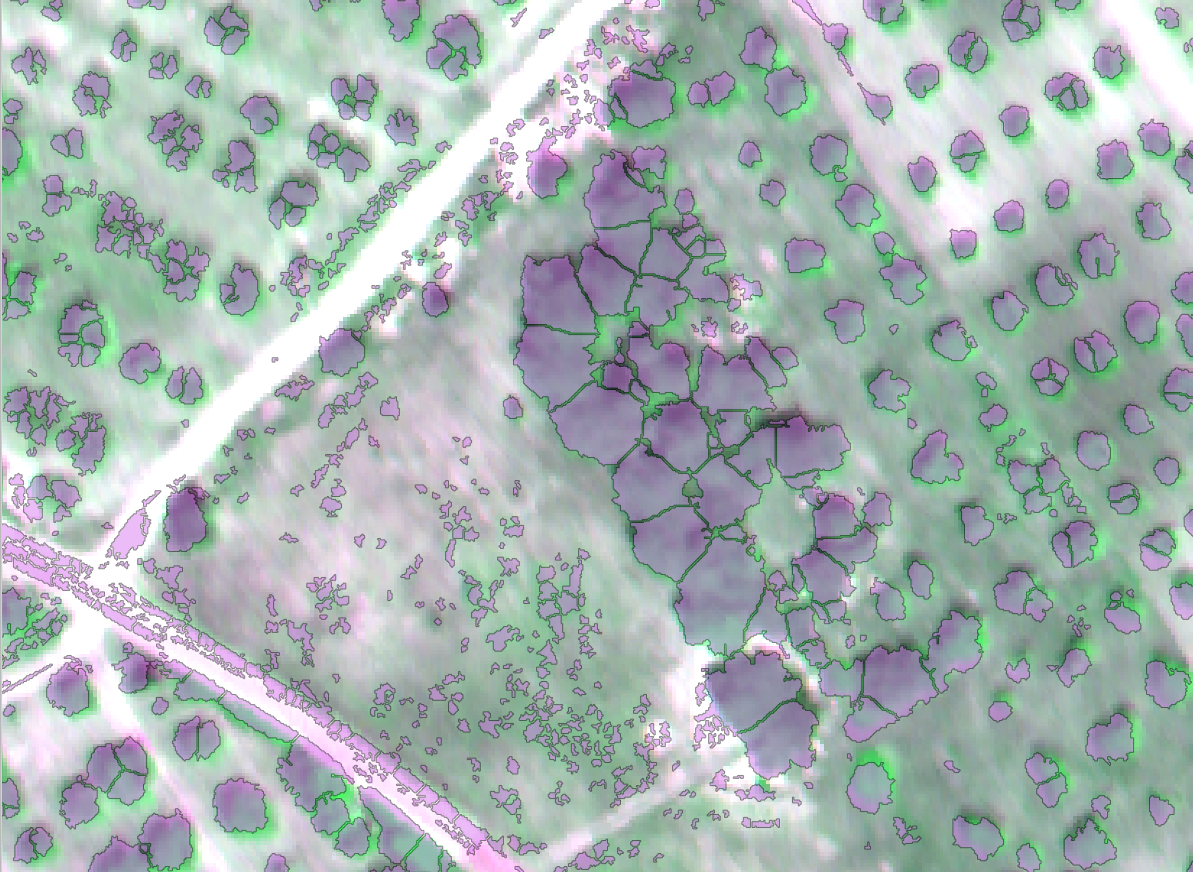
\includegraphics[height=\paperheight,width=\paperwidth]{bg_coverpage}}
\begin{frame}[plain]
\titlepage
\end{frame}}

\Large

%\begin{frame}
%  \frametitle{Processing chain}
%\begin{center}
%\begin{itemize}
% \item Fiji/ImageJ sh => Tree crowns identification NDVI-based
% \item GRASS sh => Tree crown statistics into shp file
% \item Crown Indices sh => Additional indices from refl in shp
%\end{itemize}
%\end{center}
%\end{frame}

%\transdissolve<5>
%
%\begin{frame}
%  \frametitle{GRASS script}
%\begin{center}
%\begin{itemize}
% \item GRASS7.3 in Tesla
% \item GRASS7 => RGBNIR (Acc port)
% \item GRASS7 => thermal.sh (original port)
% \item GRASS7 => rgbnir.sh (original port)
% \item \textcolor{green}{TODO: think about RGBNIR+Hyperspectral}
%\end{itemize}
%\end{center}
%\end{frame}

\transdissolve<5>

\begin{frame}
  \frametitle{Counting trees in Puglia}
\begin{center}
\begin{enumerate}
 \item Fiji watershed processing
 \item Coalescing crowns
 \item Estimating Center of crowns
 \item Merging centers
 \item Fused Crowns patches separation
 \item Merging 4\&5: Final count
\end{enumerate}
\end{center}
\end{frame}

\transdissolve<5>

{\usebackgroundtemplate{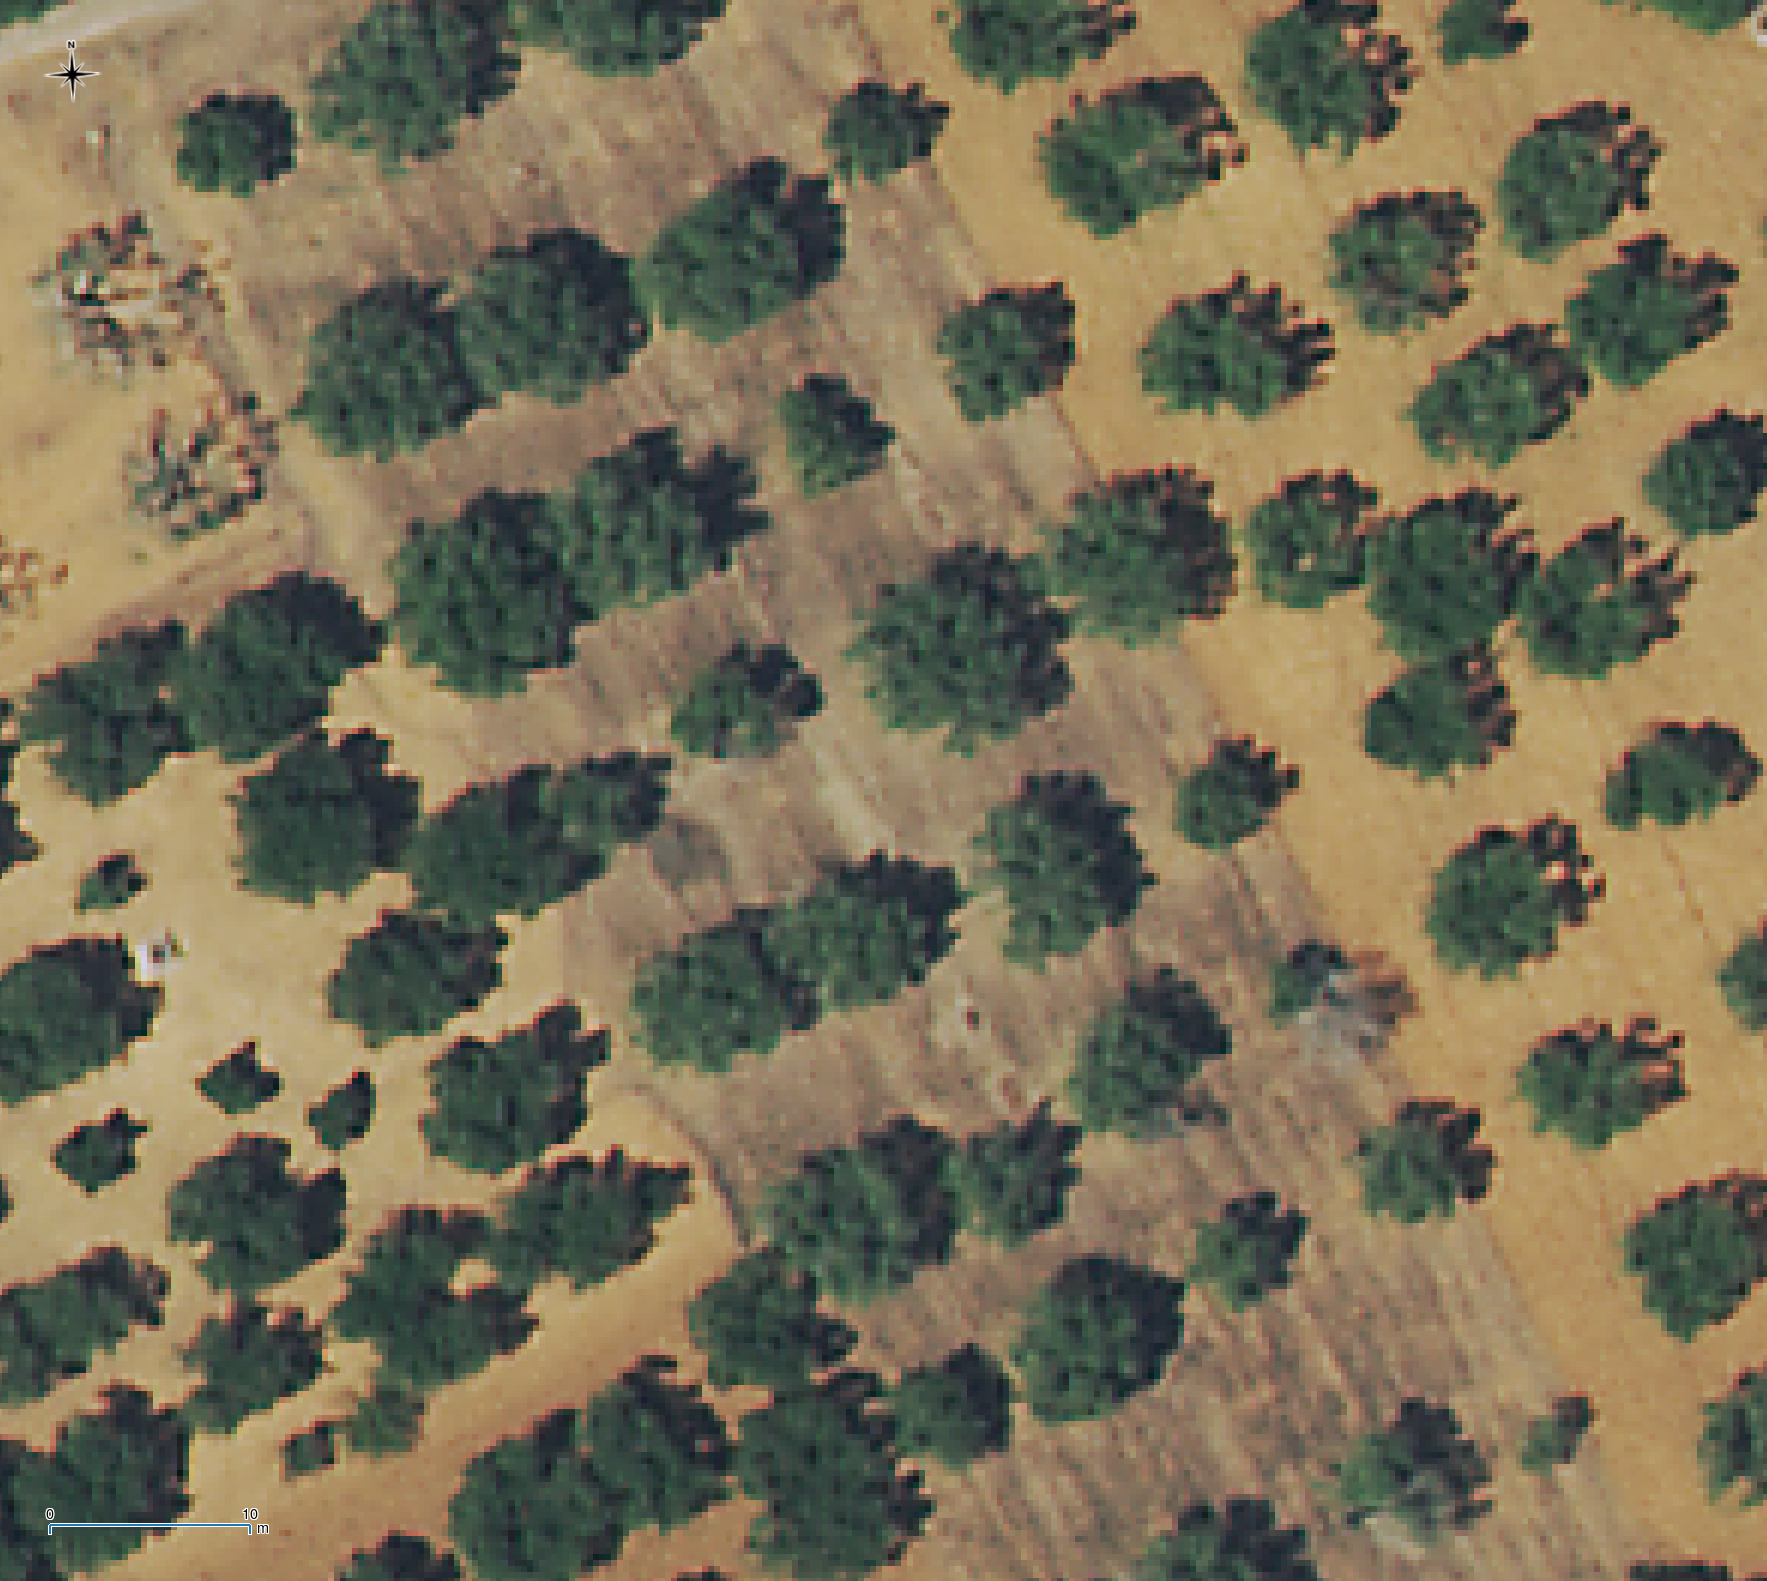
\includegraphics[height=\paperheight,width=\paperwidth]{puglia00.png}}
\begin{frame}[plain]
%\begin{shaded}
%\Huge HPC-MPI
%\end{shaded}
\end{frame}}

\transdissolve<5>

\begin{frame}
  \frametitle{1 - Fiji Watershed processing}
\begin{center}
\begin{itemize}
 \item Pablo's work
 \item Standard processing from previous work
 \item Returns a binary map 
 \item Crowns are often in clusters
\end{itemize}
\end{center}
\end{frame}

\transdissolve<5>


{\usebackgroundtemplate{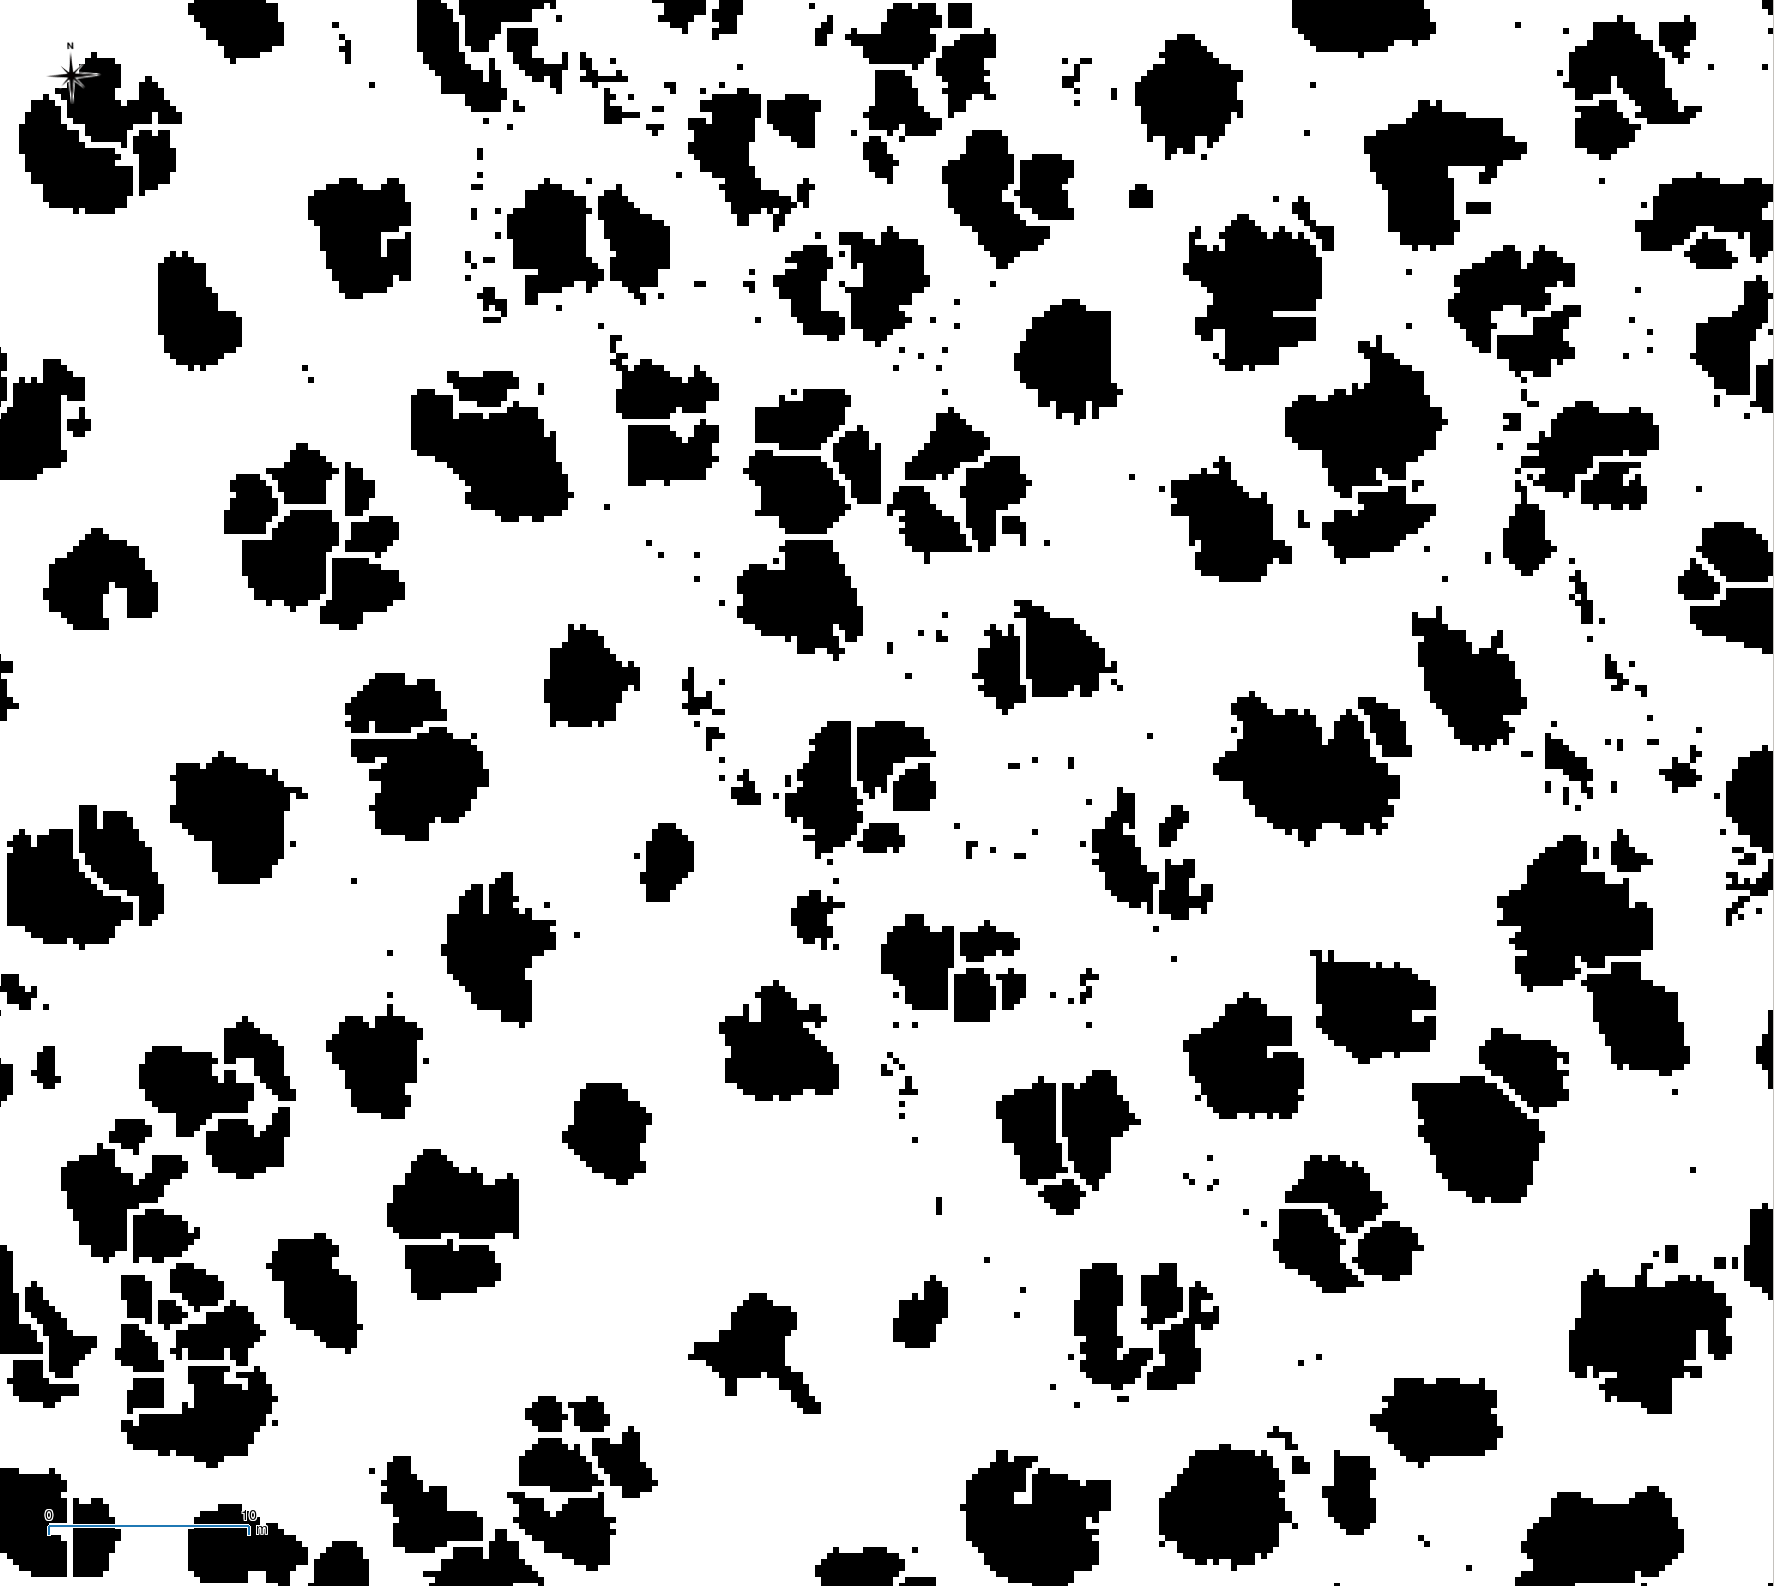
\includegraphics[height=\paperheight,width=\paperwidth]{puglia01.png}}
\begin{frame}[plain]
%\begin{shaded}
%\Huge HPC-EOSSSD
%\end{shaded}
\end{frame}}

\transdissolve<5>

\begin{frame}
  \frametitle{2 - Fill crowns}
\begin{center}
\begin{itemize}
 \item Conservative merging of crowns
 \item tries to limit possibilities of crown merging
 \item H \& V pass
\end{itemize}
\end{center}
\end{frame}

\transdissolve<5>

{\usebackgroundtemplate{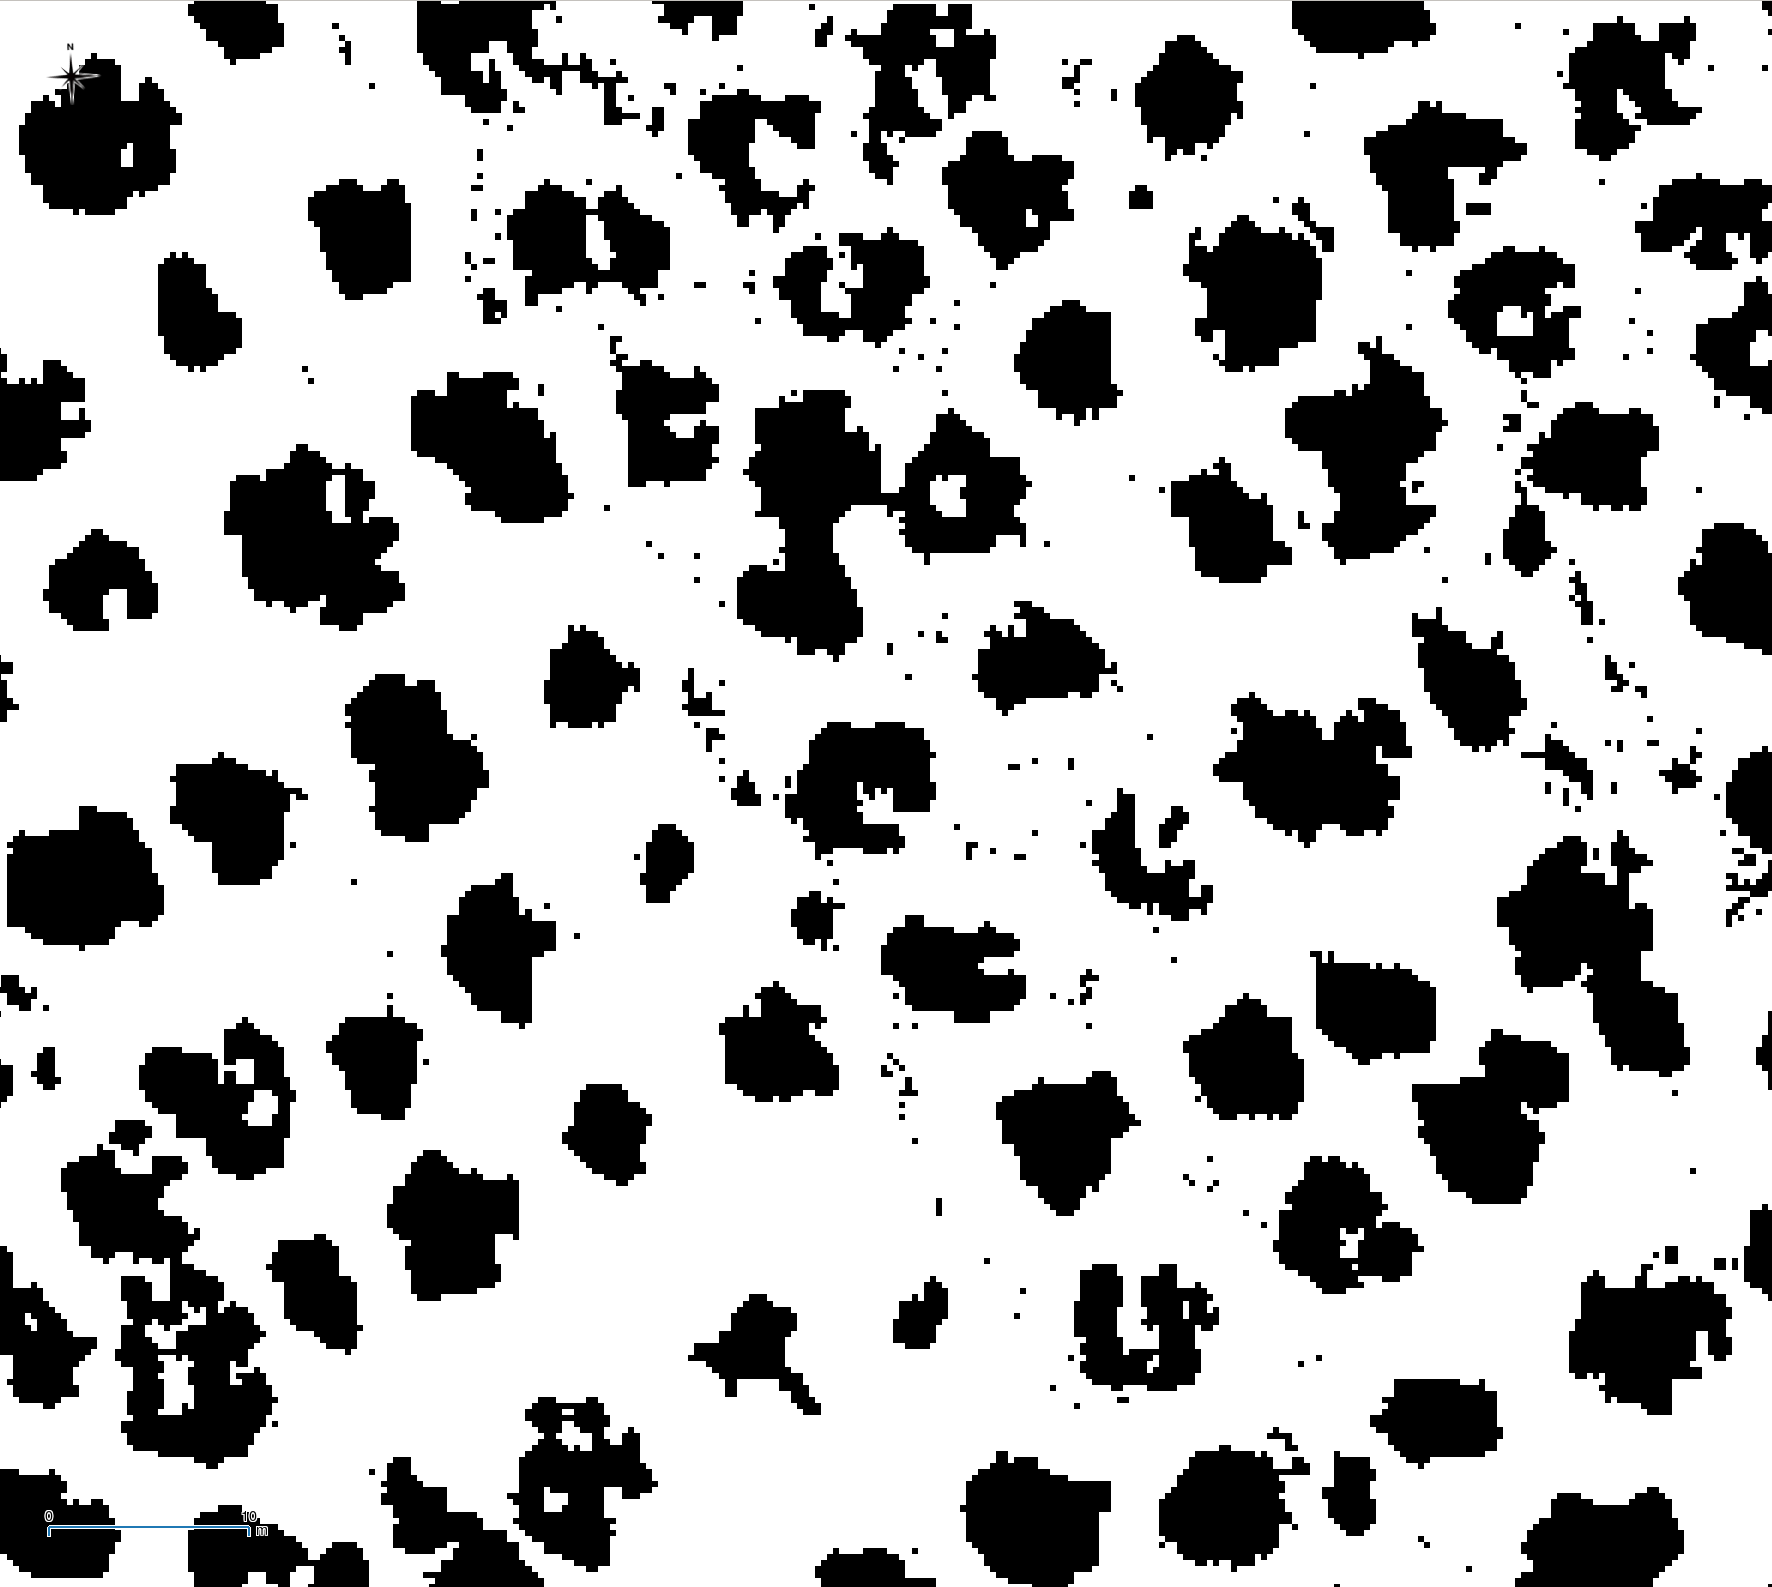
\includegraphics[height=\paperheight,width=\paperwidth]{puglia02.png}}
\begin{frame}[plain]
%\begin{shaded}
%\Huge HPC-EOSSSD
%\end{shaded}
\end{frame}}

\transdissolve<5>

\begin{frame}
  \frametitle{3 - GRASS numbering \& cleaning}
\begin{center}
\begin{itemize}
 \item Set of GRASS modules 
 \item Numbering \textit{r.clump}
 \item Area thresholding \textit{r.area}
 \item ... other manipulations to clean up stuff
\end{itemize}
\end{center}
\end{frame}

\transdissolve<5>

{\usebackgroundtemplate{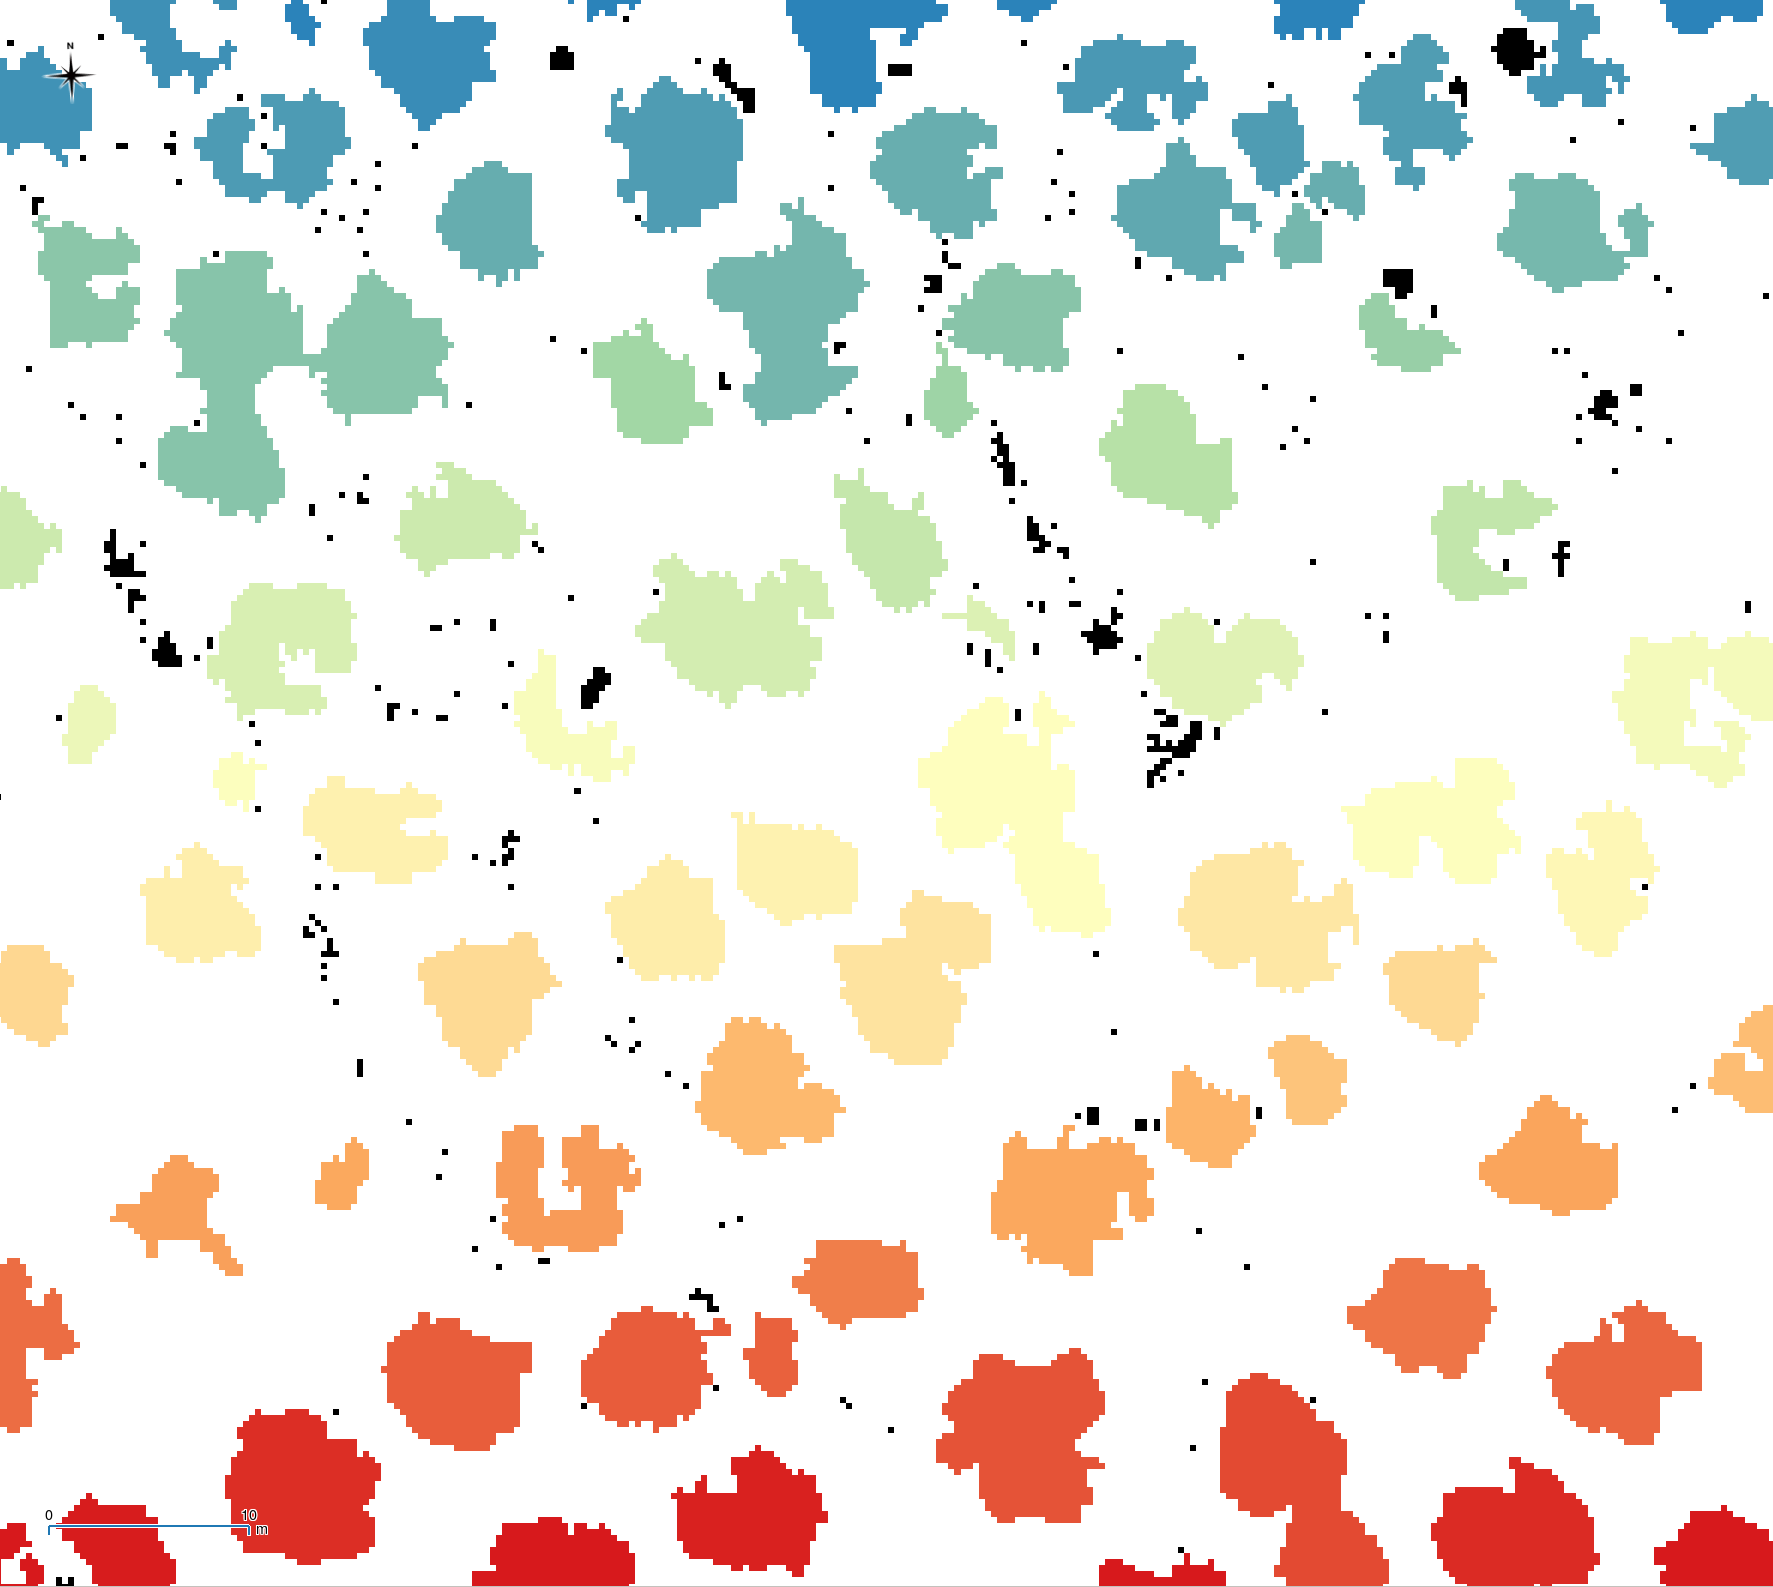
\includegraphics[height=\paperheight,width=\paperwidth]{puglia03.png}}
\begin{frame}[plain]
%\begin{shaded}
%\Huge HPC-EOSSSD
%\end{shaded}
\end{frame}}

\transdissolve<5>

\begin{frame}
  \frametitle{4 - Shape center detection}
\begin{center}
\begin{itemize}
 \item 3 points to circle method 
 \item Extensively used for all boundary members of a shape
 \item Sorting of most common center found 
 \item Used in crater manual mapping (Moon, Ceres, etc.)
\end{itemize}
\end{center}
\end{frame}

\transdissolve<5>

{\usebackgroundtemplate{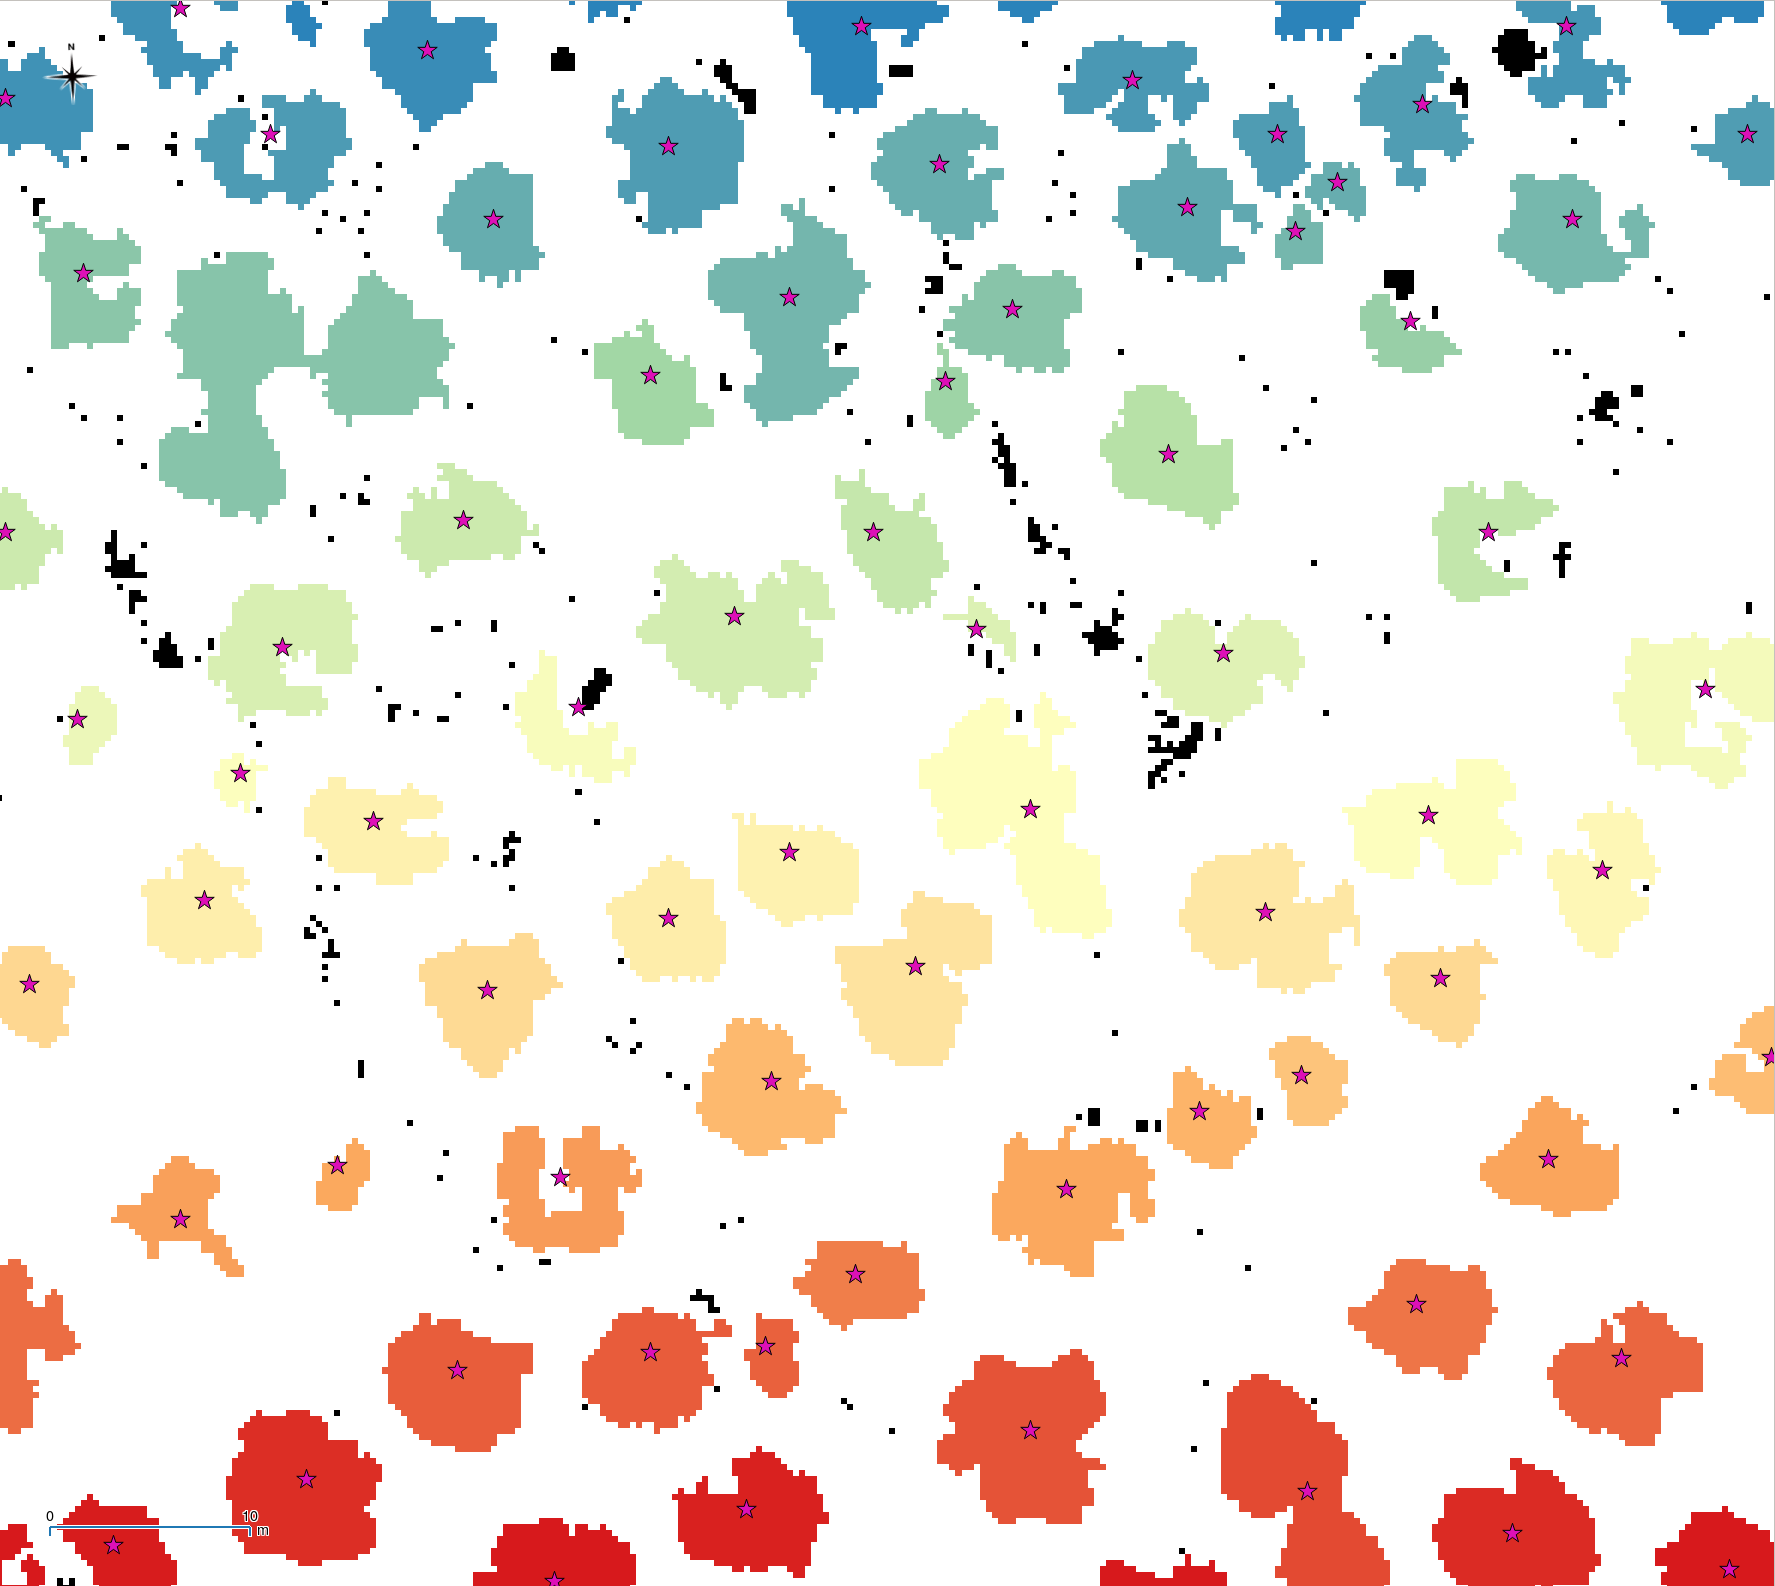
\includegraphics[height=\paperheight,width=\paperwidth]{puglia04.png}}
\begin{frame}[plain]
%\begin{shaded}
%\Huge HPC-EOSSSD
%\end{shaded}
\end{frame}}

\transdissolve<5>

\begin{frame}
  \frametitle{5 - Merge detected centers}
\begin{center}
\begin{itemize}
 \item Euclidian distance between centers 
 \item User defined threshold (i.e. 2m)
\end{itemize}
\end{center}
\end{frame}

\transdissolve<5>

{\usebackgroundtemplate{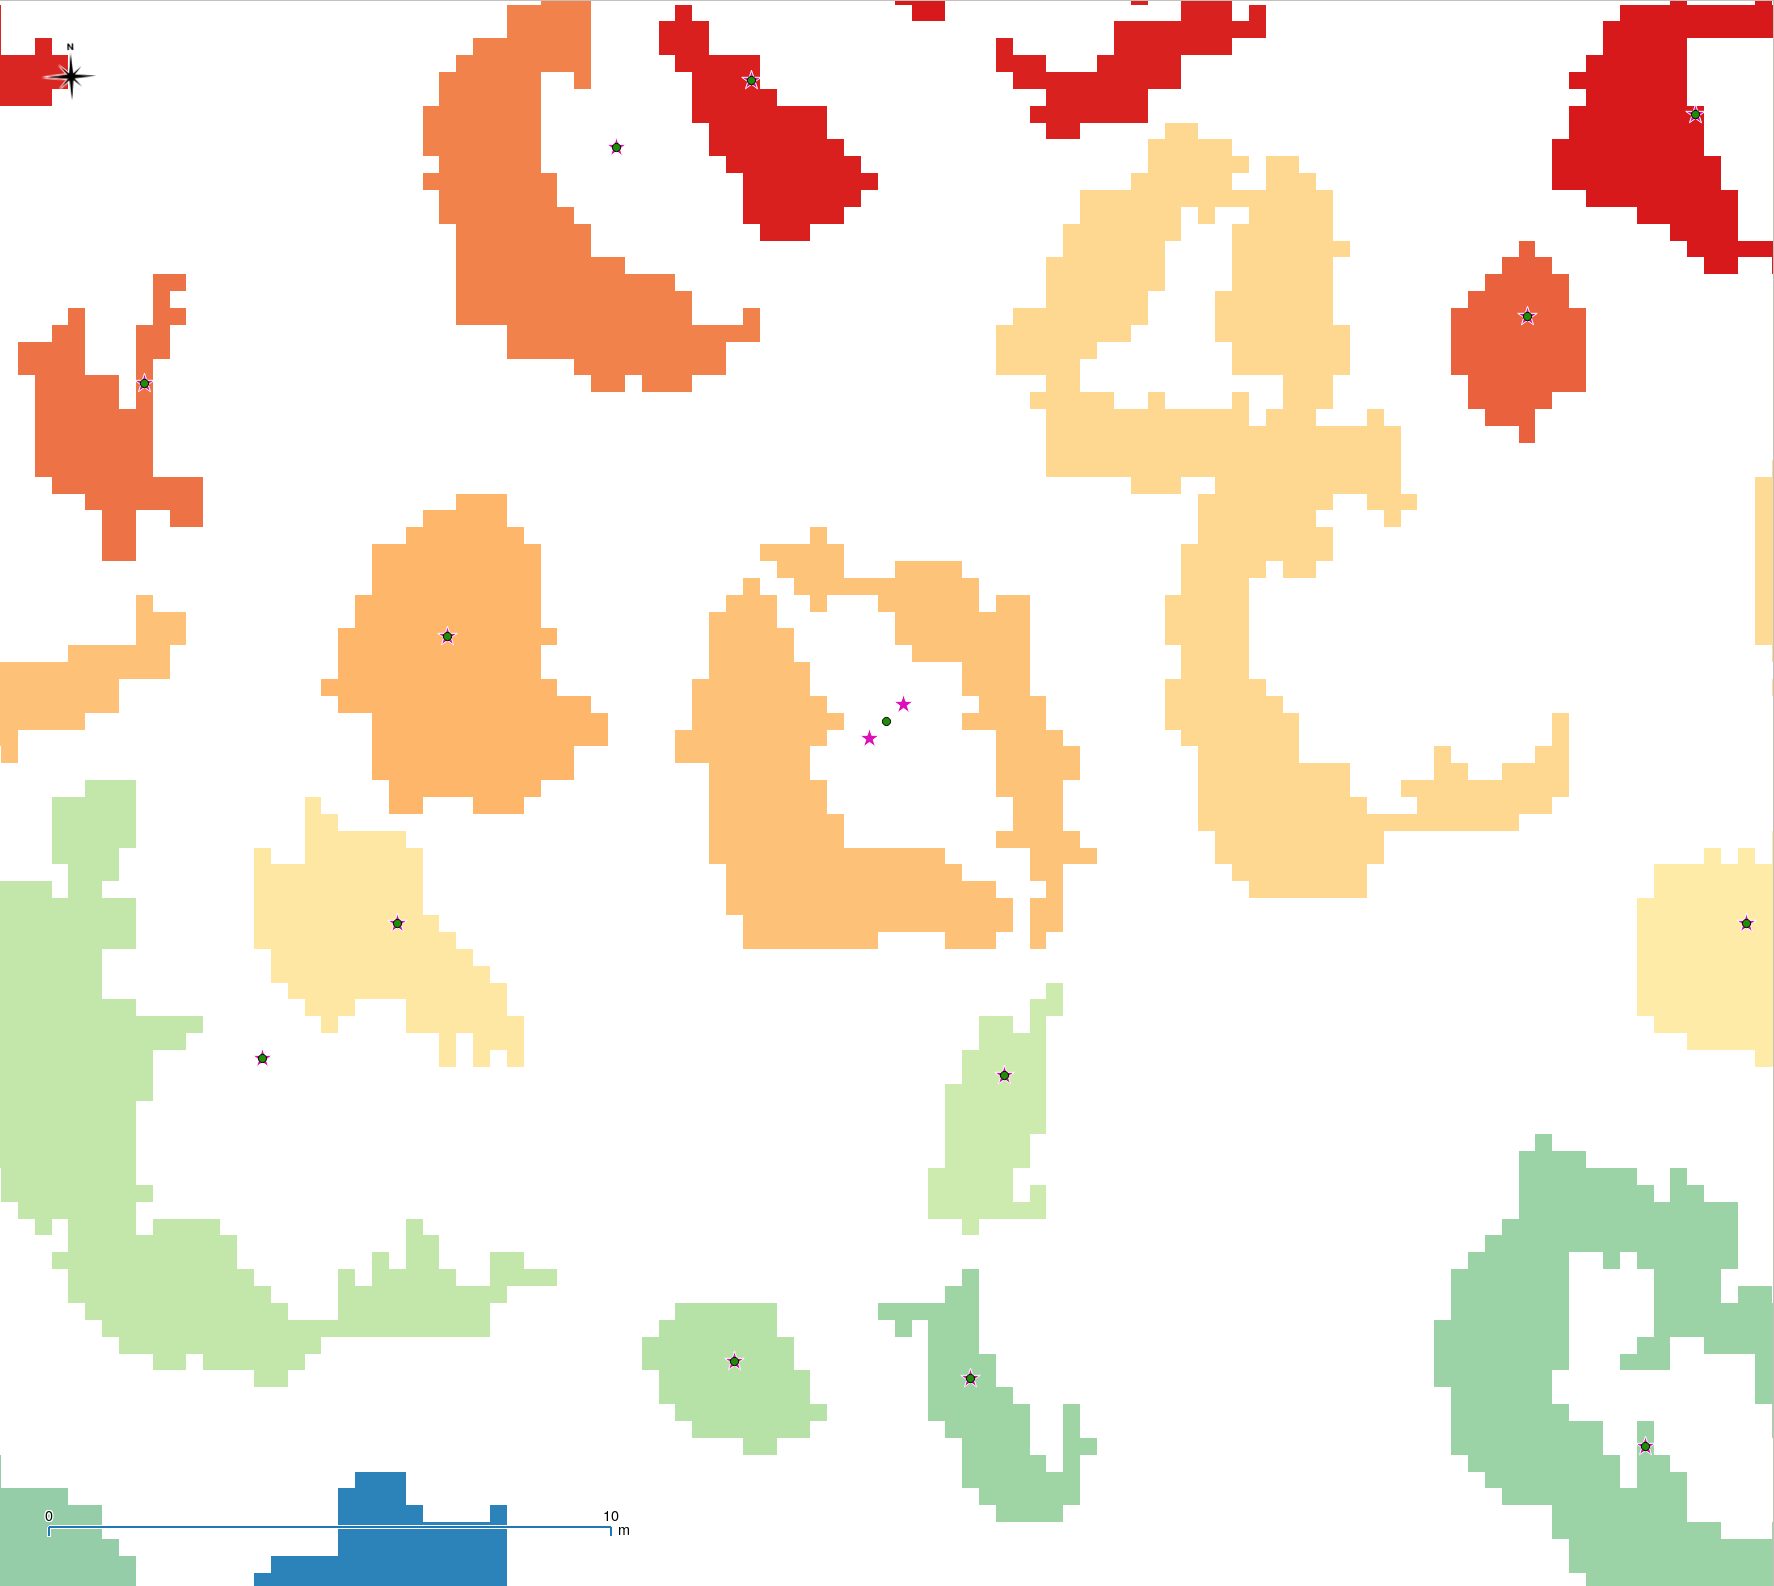
\includegraphics[height=\paperheight,width=\paperwidth]{puglia07.png}}
\begin{frame}[plain]
%\begin{shaded}
%\Huge HPC-EOSSSD
%\end{shaded}
\end{frame}}

\transdissolve<5>

\begin{frame}
  \frametitle{6 - Separate crowns}
\begin{center}
\begin{itemize}
 \item No Center for clump > 200 pixels 
 \item double crowns to multiple crowns
 \item No processing above 2000 pixels
 \item (Considered field/farmland)
 \item Mathematical Morphology
 \item Dilate, Erode, Close, Open
 \item Detect Centers
 \item Merge multiple neighbour centers
\end{itemize}
\end{center}
\end{frame}

\transdissolve<5>

{\usebackgroundtemplate{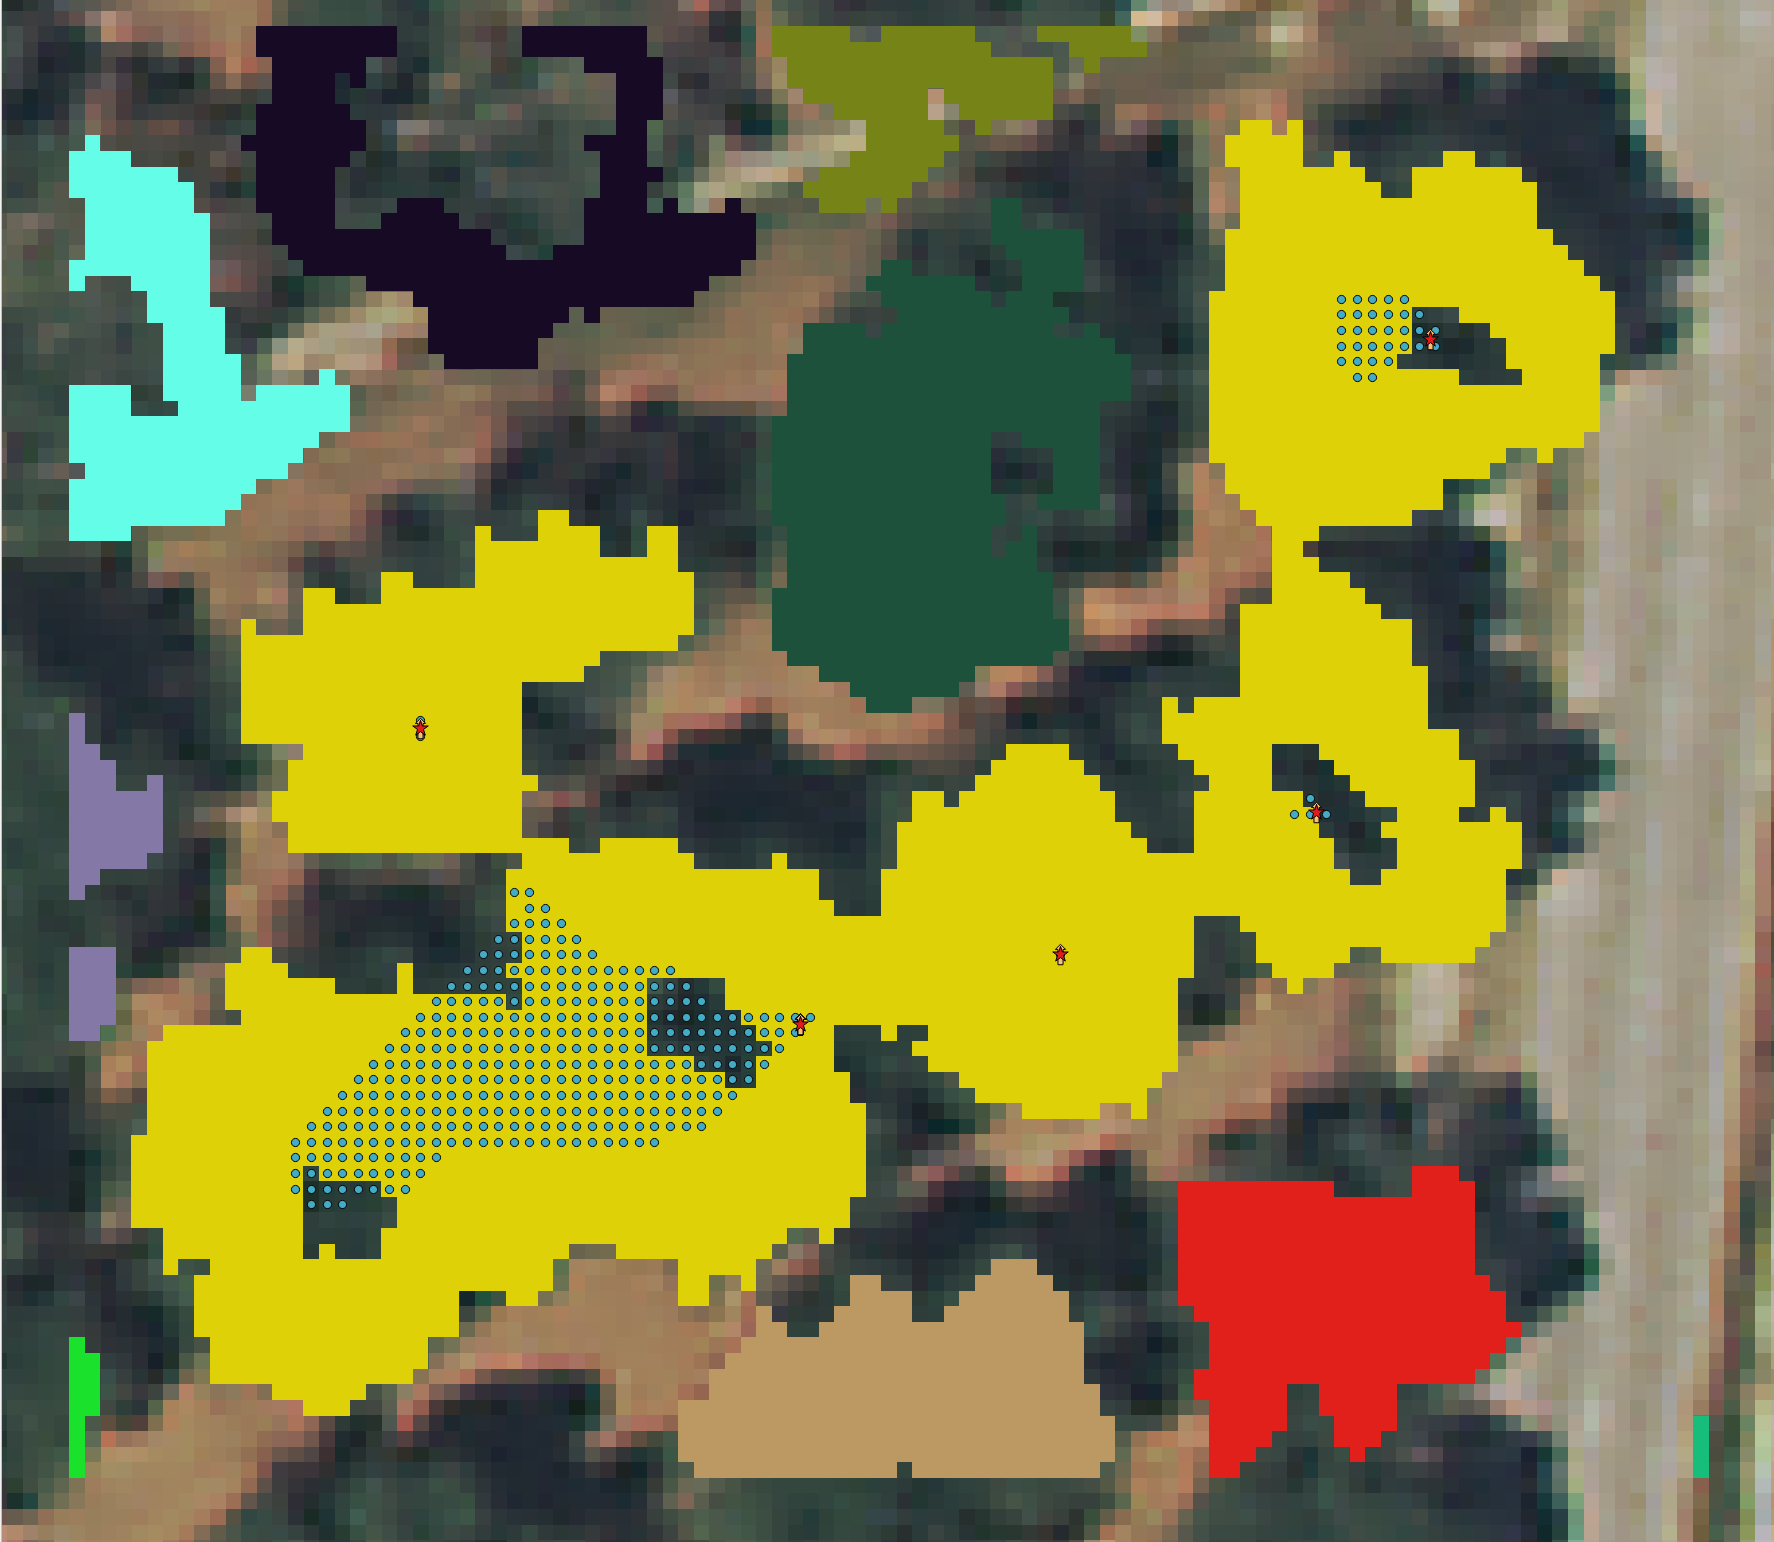
\includegraphics[height=\paperheight,width=\paperwidth]{puglia08.png}}
\begin{frame}[plain]
%\begin{shaded}
%\Huge HPC-EOSSSD
%\end{shaded}
\end{frame}}

\transdissolve<5>

\begin{frame}
  \frametitle{7 - Merge results, counting}
\begin{center}
\begin{itemize}
 \item Two sources 
 \item main: regular trees crowns
 \item Secondary: Separated tree crowns
 \item Concatenate both .csv files into one
 \item Count lines in resulting file = tree count 
\end{itemize}
\end{center}
\end{frame}

{\usebackgroundtemplate{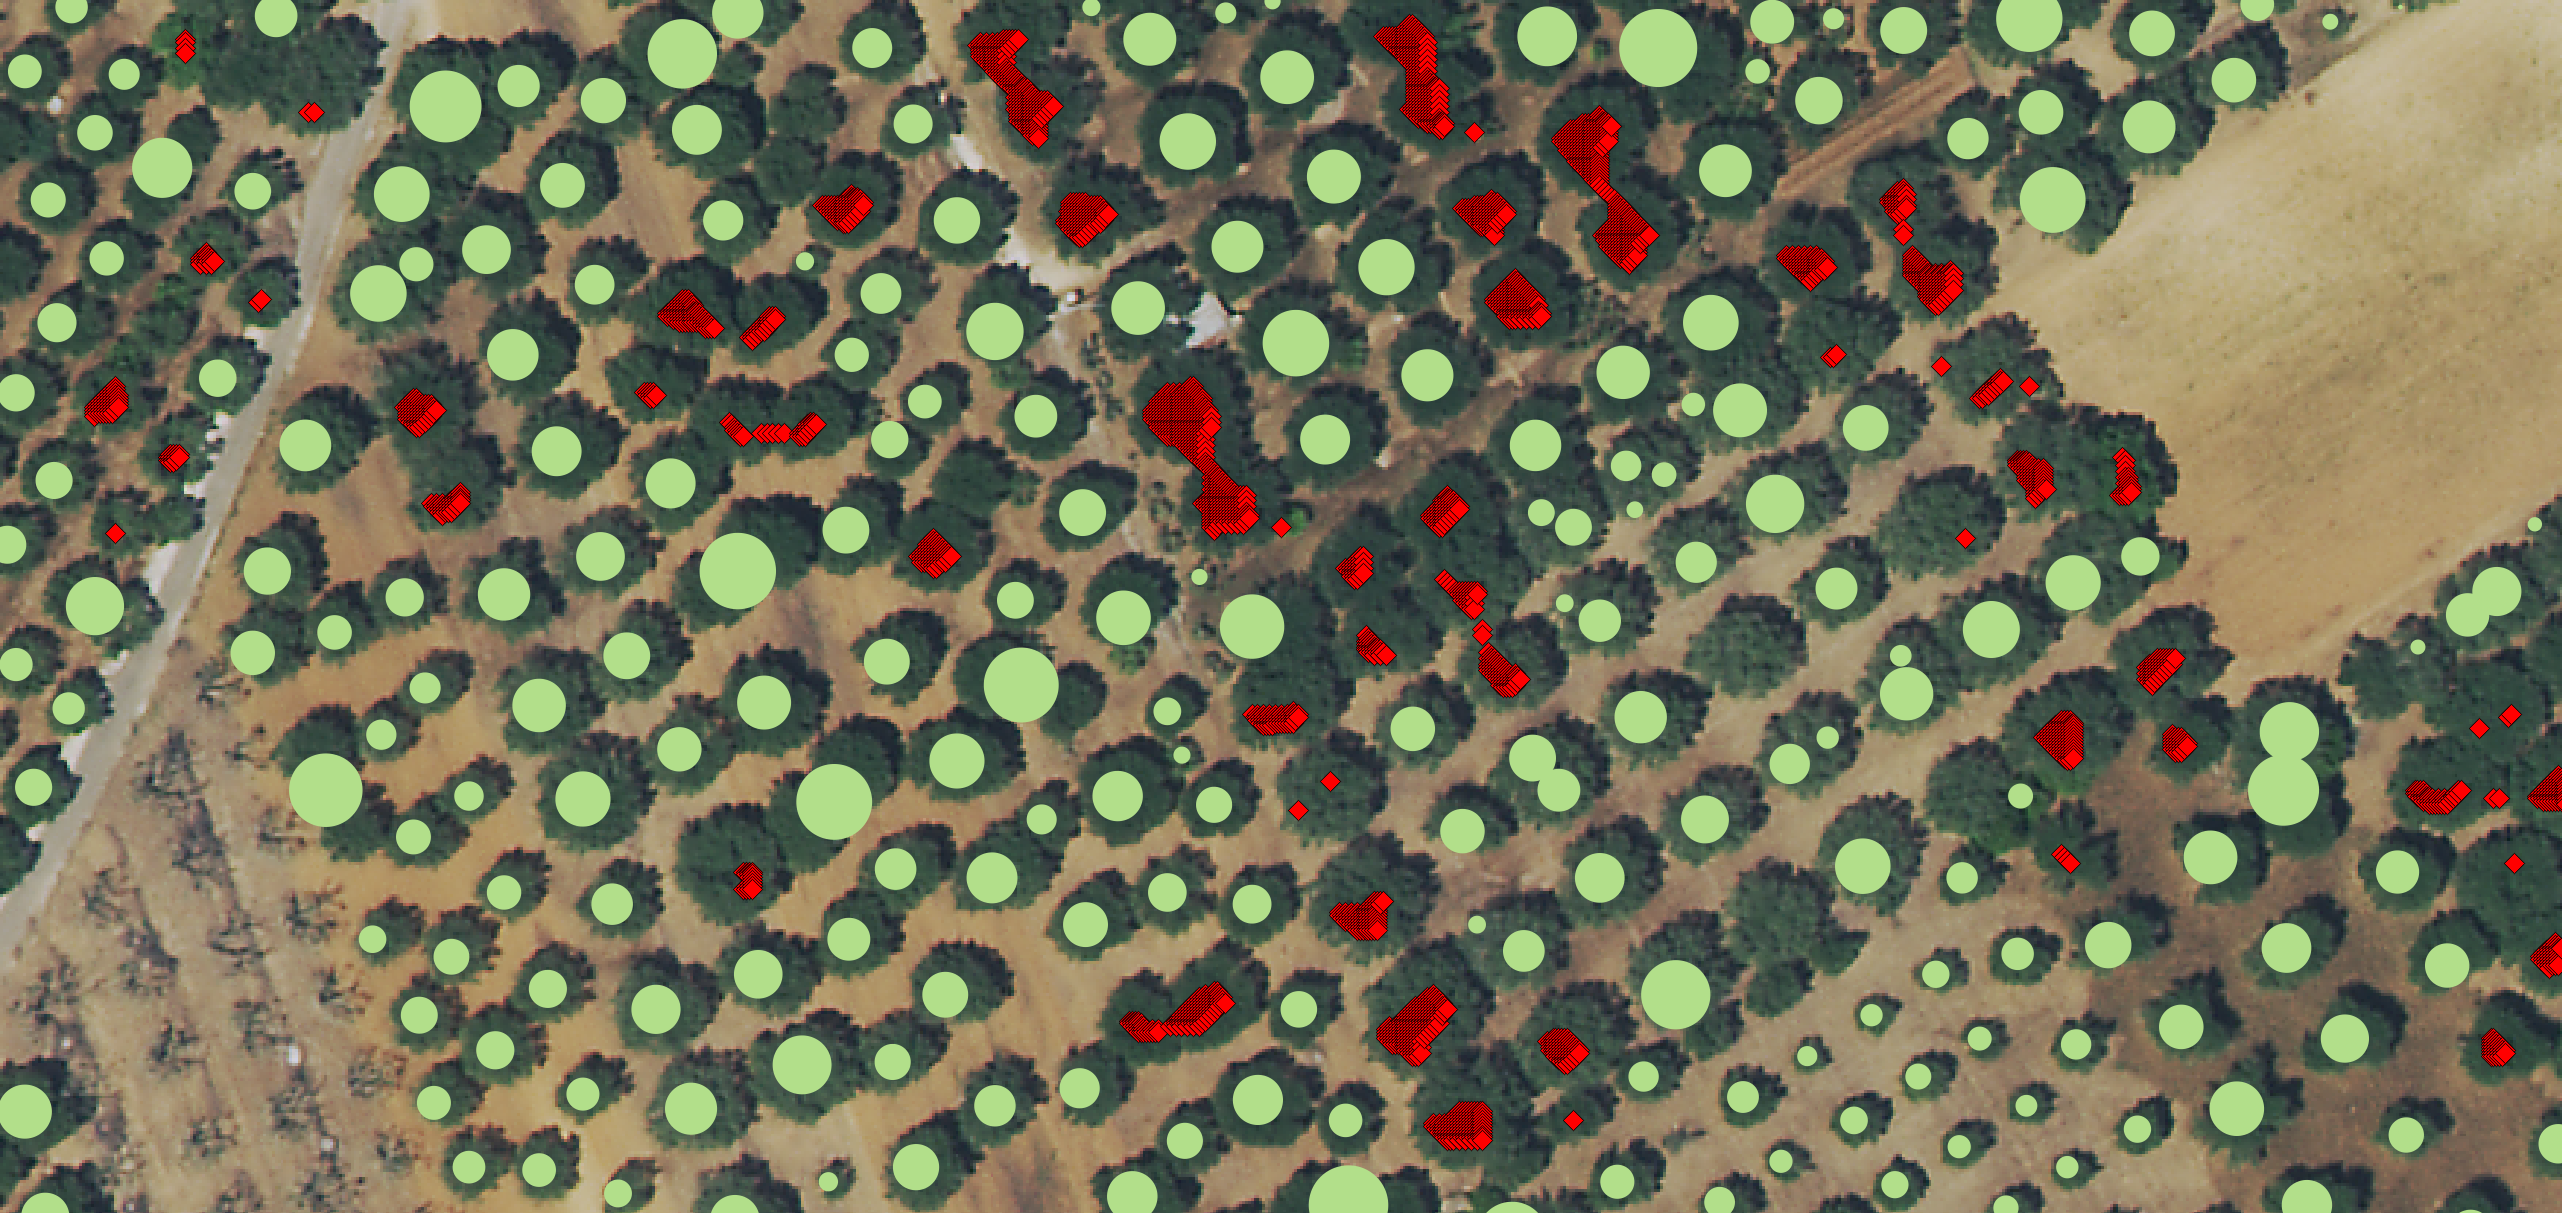
\includegraphics[height=\paperheight,width=\paperwidth]{puglia10.png}}
\begin{frame}[plain]
%\begin{shaded}
%\Huge HPC-EOSSSD
%\end{shaded}
\end{frame}}

\transdissolve<5>


%\begin{frame}
%  \frametitle{Water Level Virtual Gauge}
%\begin{columns}
%\column{0.45\textwidth}
%\begin{center}
%\begin{itemize}
 %\item Landsat Imagery
 %\item Water line
 %\item 12cm V. accuracy
 %\item 10-700Km2
 %\item Next: \\Orbital Altimetry 
%\end{itemize}
%\end{center}
%
%\column{0.5\textwidth}
%\begin{center}
% 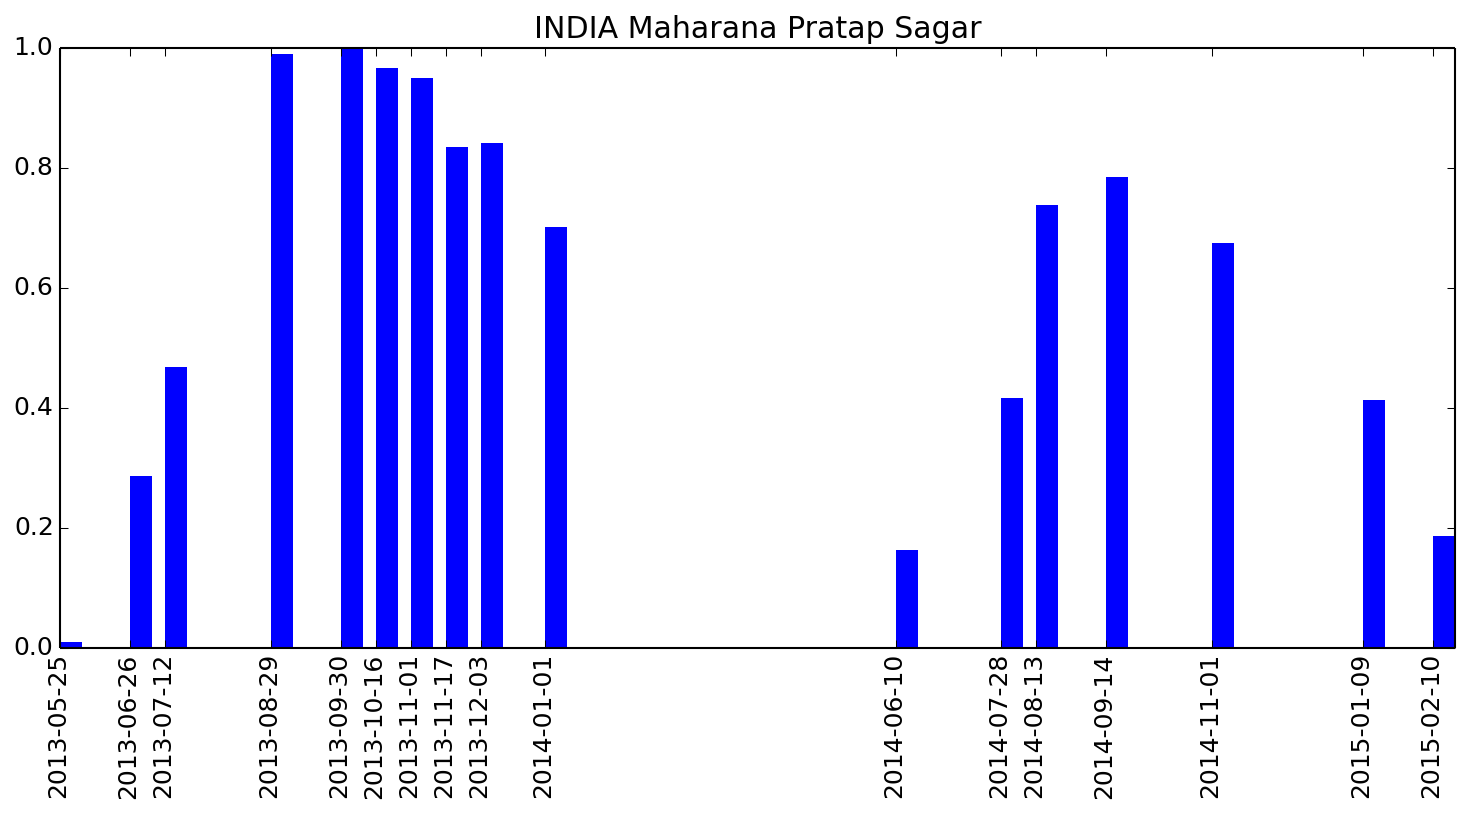
\includegraphics[height=3cm]{IN_Maharana_Pratap_Sagar_wLVG1}
% %\includegraphics[height=2.5cm]{PK_TarbelaDam_wLVG1)\\
% %\includegraphics[height=3cm]{EG_AswanDam}
%\end{center}
%\end{columns}
%\end{frame}

%\transdissolve<5>

%\begin{frame}
%  \frametitle{Equations}
%  Equations are easy
%  \begin{itemize}
%  \item Just copy and paste equations\pause
%  \item From the paper!
%    \begin{equation*}
%      \textbf{p}^* = \underset{\textbf{p}}{\arg\!\min}~\sum_{\textbf{x}}\left[ I(\textbf{W}(\textbf{x};\textbf{p})) - T(\textbf{x}) \right]^2
%    \end{equation*}
%  \end{itemize}
%\end{frame}
%
%\transdissolve<5>

%\begin{frame}
%  \frametitle{A Movie}
%  \begin{center}
%    \movie[height=5cm,width=6.5cm,poster,autostart,loop]{}{video1.avi}
%  \end{center}
%  \begin{itemize}
%  \item Movies only seem to work in Adobe Reader
%  \item Movie file is not embedded, it must be on the computer
%  \end{itemize}
%\end{frame}

%\transdissolve<5>

{\usebackgroundtemplate{\includegraphics[height=\paperheight,width=\paperwidth]{puglia09.png}}
\begin{frame}[plain]
\begin{shaded}
\Huge Thank you
\end{shaded}
\end{frame}}
\end{document}
